% !TEX TS-program = xelatex
% !TEX encoding = UTF-8 Unicode

% \documentclass[AutoFakeBold]{LZUThesis}
\documentclass[AutoFakeBold]{LZUThesis}

\begin{document}
%=====%
%
%封皮页填写内容
%
%=====%

% 标题样式 使用 \title{{}}; 使用时必须保证至少两个外侧括号
%  如: 短标题 \title{{第一行}},  
% 	      长标题 \title{{第一行}{第二行}}
%             超长标题\tiitle{{第一行}{...}{第N行}}

\title{{基于 CEEMDAN 多特征分解和}{Prophet 与 GRU 组合模型预测短期风速}}



% 标题样式 使用 \entitle{{}}; 使用时必须保证至少两个外侧括号
%  如: 短标题 \entitle{{First row}},  
% 	      长标题 \entitle{{First row}{ Second row}}
%             超长标题\entitle{{First row}{...}{ Next N row}}
% 注意:  英文标题多行时 需要在开头加个空格 防止摘要标题处英语单词粘连。
\entitle{{Forecast Short-term Wind Speed through CEEMDAN}{ Decomposed Multi-features and Prophet \& GRU Hybrid Model}}

\author{蒋嵩林}
\major{计算机科学与技术(基础理论班)}
\advisor{任超}
\college{信息科学与工程学院}
\grade{2018级}



\maketitle

%==============================%
% ↓ ↓ ↓ 诚信说明页 授权说明书
%==============================%

% 1. 可以调整签字的宽度,现在是40
% 2. 去掉raisebox的相关注释(注意上下大括号对应),可以改变-5那个数字调整签名和横线的上下位置

% 你的签名,signature.pdf 改为你的签名文件名,
\mysignature{
    % \raisebox{-5pt}{
        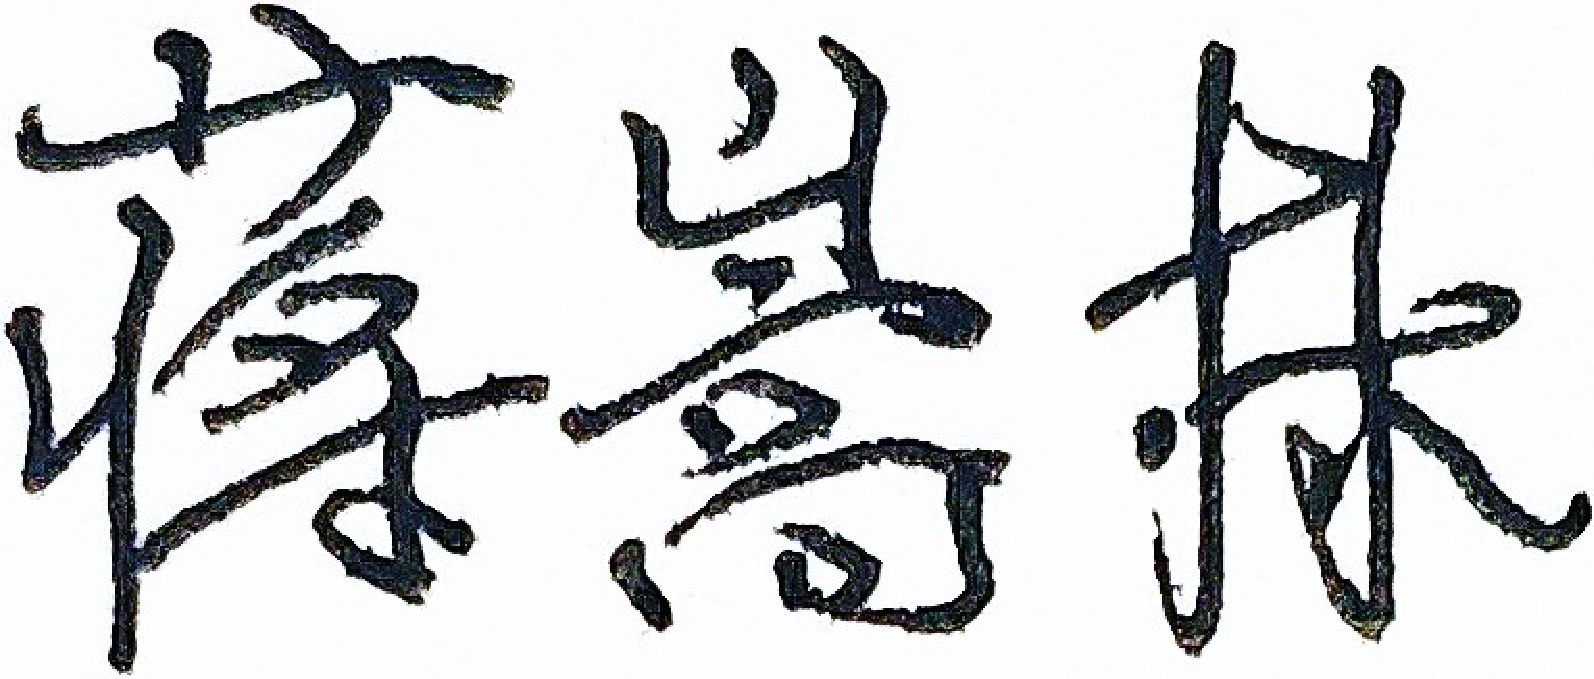
\includegraphics[width=60pt]{author_sig.pdf}
    % }
}
% % 你手写的日期,signature.pdf 改为你的手写的日期文件名
% \mytime{
%     % \raisebox{-5pt}{
%         \includegraphics[width=40pt]{signature.pdf}
%     % }
% }
% % 老师的手写签名,signature.pdf 改为老师的手写签名文件名
% \supervisorsignature{
%     % \raisebox{-5pt}{
%         \includegraphics[width=40pt]{signature.pdf}
%     % }
% }
% % 老师手写的时间,signature.pdf 改为老师的手写的日期文件名
% \teachertime{
%     % \raisebox{-5pSt}{
%         \includegraphics[width=40pt]{signature.pdf}
%     % }
% }
% % 老师手写的成绩
% \recommendedgrade{
%     % \raisebox{-5pt}{
%         \includegraphics[width=40pt]{signature.pdf}
%     % }
% }

\makestatement

%==============================%
% ↑ ↑ ↑ 诚信说明页 授权说明书
%==============================%


%=====%
%论文(设计)成绩:注意2007的模板要求,成绩页在最后,2021要求成绩页在摘要前面
%=====%

% 下面这些注释掉可以去掉成绩、评语什么的
\supervisorcomment{}


\committeecomment{}

\finalgrade{}
% 上面这些注释掉可以去掉成绩、评语什么的

\Grade %这一句才是成绩页,上面是填写


\frontmatter



%中文摘要
\ZhAbstract{
气候变化和环保问题关乎人类未来命运。在石油危机以及全球变暖问题愈发严重的现在,
可再生清洁能源相关研究成为了学界的关注热点。风能,作为触手可得的一种能源,正成为新能
源的主力军之一。准确预测风速,从而保证电网的稳定性,具有十分重大的意义。风速预测
是一个时间序列回归问题,由于风速的波动具有随机性,其影响因素也十分复杂,呈现出
非平稳且非线性的特征,因而对短期风速的预测难度较大。

本文选取数值天气预报中常见的六种气象要素历史数据,包括近地面气温、近地面气压、
近地面空气比湿、地面向下短波辐射、地面向下长波辐射、地面降水率,结合近地面全
风速的历史数据构建短期风速的预测模型。首先,采用当前科研最前沿的自适应噪声完备
集合经验模态分解(CEEMDAN)算法,对上述七种特征历史数据进行分解,将高频噪声和
低频信号进行分离,降低时间序列数据分析的复杂度,从而提高准确性。然后,将分解结
果序列输入由 Facebook 推出的主流时间序列预测框架 Prophet 进行预测以及统计分
析,得到Prophet拟合预测的结果以及统计分析预测得出的趋势分量、累加式季节性分量
、日分量、年分量以及上述分量所对应的预测最大边界和最小边界,进一步降低七种特征
对应时间序列的复杂度,便于神经网络的训练。最终,将所有由 Prophet 分析预测的时
段对应的结果以及分量输入进一个由三层门控循环单元(GRU)构成的深度学习模型,采
用最新科研成果 Nadam 优化器 以及 Huber损失函数训练模型,输出预测的时段对应的
近地面全风速,从而达成预测实际的短期风速的目的。

为了验证模型的实际效果,本文选取了甘肃中电酒泉第四风力发电有限公司附近(北纬
40.65 度,东经 96.95 度)的2017年1月1日0时整至2018年12月31日21时整
\footnote{此处所述时间均为协调世界时(UTC, Universal Time Coordinated)。}间
隔三小时的历史数据,使用均方误差(MSE)、平均绝对误差(MAE)、平均绝对误
差百分比(MAPE)、均方根误差(RMSE)、决定系数($R^2$)等多项指标,以及对模型的预
测结果进行可视化分析,与只使用近地面全风速历史数据、未进行时间序列分解剔除噪声、
只使用单一模型的情况进行对比,对模型全方面综合评估。结果表明,使用本文提出的模型
,预测短期风速的精度会明显提升,因而具有优越性。
}{风速影响因素,短期风速预测,组合模型,自适应噪声完备集合经验模态分解,Prophet,门控循环单元神经网络,深度学习,数据科学}


%英文摘要
\EnAbstract{\fontspec{Times New Roman} {
Climate change and environmental issues matter the destiny of mankind. 
With the oil crisis and global warming becoming more and more serious,
renewable energy related research has become a hot spot which
attracts great attention from academic. Wind, as a readily available 
energy source, is becoming the mainstream in renewable energy. As a result,
it is of great significance to accurately predict the wind speed
so that power system stability can be ensured. Wind speed forecast
is a time series regression problem. Due to the randomness of wind
speed fluctuations, influencing factors for wind speed are very complex,
which shows its characteristics of non-stationary and nonlinear, so it is 
difficult to predict short-term wind speed.

This paper selects the historical data of six common meteorological
elements in numerical weather prediction, including near-surface air 
temperature, near-surface air pressure, near-surface specific humidity,
surface downwelling shortwave radiation, surface downwelling longwave
radiation, and surface precipitation rate. Combine historical time series
data of near-surface total wind speed with the above mentioned elements
and build the short-term wind speed forecasting model. Firstly, CEEMDAN
(Complete Ensemble Empirical Mode Decomposition with Adaptive Noise) 
algorithm, which is at the forefront of current scientific research,
is used to decompose the above seven elements' historical data so that
high-frequency noise and low-frequency signals can be separated, which
eventually leads to reduction of the complexity of time series data
analysis, and improving accuracy. Then, input the decomposed sequence
into Prophet, a mainstream time series forecasting framework developed by
Facebook, for forecasting and statistical analysis, and obtain the
result of Prophet fitting prediction, the trend component, additive
seasonality component, daily component, yearly component as well as
maximum and minimum boundaries of above. These features further help
reduce the complexity of the time series corresponding to the seven
meteorological elements and facilitate the training of the neural
network. Finally, all the predictions and components corresponding
to the time series elements predicted by the Prophet analysis are input
into a deep learning model composed of a three-layer Gated Recurrent Unit
(GRU). Use the latest scientific research results Nadam optimizer and
Huber loss function to train the model, and output the near-surface
total wind speed corresponding to the predicted time period, so that
the actual short-term wind speed can be predicted.

In order to verify the actual effect of the model, this paper selects the
historical data at a location near Gansu Zhongdian Jiuquan Fourth Wind
Power Co., Ltd. (latitude 40.65 degrees north, longitude 96.95 degrees
east) from 0:00 on January 1, 2017 to 21:00 on December 31, 2018 
\footnote{The times mentioned here are all in UTC (Universal Time Coordinated). } 
at three-hour intervals, using various evaluating indicators like
Mean Squared Error (MSE), Mean Absolute Error (MAE), Mean Absolute
Percentage Error (MAPE), Root Mean Squared Error (RMSE), Coefficient of
Determination ($R^2$), etc. The predicted results are visualized, and 
make comparison with the case of only using the near-ground full wind
speed historical data, without time series decomposition to remove
noise, and only using a single model, the model is comprehensively
evaluated in all aspects. The results show that using the model
proposed in this paper, the accuracy of predicting short-term
wind speed will be significantly improved, so it has supremacy.
}}
{wind speed influencing factors; short-term wind speed forecast; 
hybrid model; CEEMDAN; Prophet; GRU; deep learning; data science.
}

%生成目录
\tableofcontents
% \thispagestyle{empty}


%文章主体
\mainmatter

\chapter{绪 \qquad 论}

% !学校要求的规范,绪论是单独的,不是第一章,但是老师们都是让作为第一章,这里我把它放在了论文里,如果你要让在外面,只需要把上面的 \mainmatter 这一句话放在“绪论内容后面,正文第一章前面”即可,也就是 \chapter{latex部分用法简介} 这一句话上面

% \Intro{
\section{选题研究背景及意义}
\subsection{风力发电的前景}
随着工业发展的需要,人类社会对能源的依赖度也在逐步上升。第二次能源革命以来,
传统化石燃料的使用导致了一系列的问题。化石燃料在开采过程中也产生了
一系列的环境问题。以煤炭为例,在开采时,会破坏地表原本的性状,引发滑坡,塌陷
等一系列问题。开采煤炭所产生的废渣也难以处理,产生的污水会对水土环境造成污染。
同时,燃烧化石燃料所产生的二氧化硫($SO_2$)和氮氧化物会形成酸雨、粉尘使空气能
见度降低、一氧化碳(CO)和芳香烃化合物会污染空气。二氧化碳($CO_2$)在大气层中所
占比例的提高,也导致了温室效应与气候变化,从而使得一些极端天气灾害的发生频率
有了显著的升高。然而目前,在世界能源消费占比中,煤炭和石油的比重仍较重要。
我国的能源生产和消费构成中,煤炭在2019年仍在一次能源中占比57.7\%,占据着
主要地位。\cite{能源数据2021王庆一}

当前传统化石燃料,由于其储量的有限性,也正逐步面临枯竭的风险。“绿水青山就
是金山银山”。可再生能源的发展,不仅将会确保绿水青山的存在,而且同时也必然即
将成为金山银山的重要组成部分。过去三十年以来,风能一直保持着最快增长的可再
生能源的记录,是目前全球第二大的可再生能源。风能本质上属于一种气象能源,其
为太阳照射环境下地球表面受热不均,在水平气压梯度力的影响下,由于温差造成大
气对流所产生的一种能量来源。有相关研究
\cite{李仲蔚2019风力发电企业价值评估研究}估算结果表明,全球可开发
利用的风能资源达到了二百万兆瓦($2\times10^7MW$),是目前全球第一大的可再生
能源水能的10倍。风能因其分布广泛,弥补了水能发电需要的苛刻条件以及对生态自
然环境可能造成不良影响的缺陷。如将预估的可利用风能的1\%加以利用,即可以满
足全球能源的发电使用需求,因而发展潜力极其巨大,十分有望在将来替代水能成为
全球第二大的可再生能源。

\subsection{短期风速预测的意义}
短期风速的主要影响因素分为气象因素和地形因素。其中,气象因素主要包括温度、气压、
湿度等,而地形因素包括地貌、地表障碍等\cite{王秀2021基于} 。

对于短期近地面风速的预测能够很好的帮助并促进风能的应用。首先,风力发电厂管理人员
可以通过预测结果优化电力分配,提高发电量;其次,风力发电厂还可以准确的在风速
过大之前对风力发电机指示停机,预防风力发电机的过载损毁,避免或者减少相应的损
失;最后,还可以有效安排好风力发电的电网并网问题,减少因为风速的剧烈波动对电
网电业的稳定性影响,降低运营成本,增加风电场的效益。

对于目前的风速预测研究而言,相关问题主流使用的模型包括传统时间序列模型以及
深度学习模型。他们各自都存在一定的优点和缺陷,单一模型并不能很好的进行预测
\cite{陆冰鉴2020基于}。同时,由于风速数据中往往包含着较大的噪声问题,如何
有效地对其数据集进行降噪处理也是目前研究的方向。由于单一的预测方法无法做到
很好的风速预测,如果能通过组合模型,对其进行精确的预测,将会对风力发电的应
用起到巨大的促进作用。

\section{选题已有研究成果综述}
\subsection{数值预报方法}
数值预报方法使用大气压、气温、相对湿度、风速等数值型数据来作为初始状态,
以流体力学方程和热力学方程为依据来实现整个大气状态模型的构建,通过超级
计算机进行数值计算求解,得到未来天气的预报结果。
\cite{姜兆宇2019多时空尺度的风力发电预测方法综述}

目前数值预报方法已经很成熟,准确性良好,已经广泛地应用到了天气预报中。
但是,由于数值方法需要占用大量的计算资源,难以将时间和空间分辨率
都做得很高,因而数值预报一般不适用于短期风速预报。

\subsection{传统机器学习方法}

\subsection{深度学习方法}

\subsection{降噪方法}
% }


% % =======正文从第一章开始
% \setcounter{chapter}{0}

\chapter{数据来源及特征选取}

这里写这一章节的内容

\section{这里是二级标题}
这里是文章内容

\subsection{这里是三级标题}
这里是文章内容

\chapter{使用方法介绍}

\chapter{模型的建立和评估}

\chapter{总结与展望}

%论文后部
\backmatter


%=======%
%引入参考文献文件
%=======%
\bibdatabase{bib/database}%bib文件名称 仅修改bib/ 后部分
\printbib
% \nocite{*} %显示数据库中有的,但是正文没有引用的文献


\Appendix


这里是附录页,附上你的程序或必要的相关知识

{\bfseries 编译方式:} XeLaTeX -->BibTeX --> XeLaTeX-->XeLaTeX



\Thanks

本文在写作时从GitHub中获取并使用了兰州大学2016级物理科学与技术学院本科生余航
制作的“兰州大学本科生2021学士学位毕业论文LaTeX模板”,在此也一并致谢。

\end{document}